\chapter{Box Plot e Histograma}

    \setcounter{section}{0}

    Com as categorias das variáveis colocadas, é possível inserir agora os dados coletados em gráficos, para 
    analisar tais dados em conjunto. O primeiro gráfico utilizado é o chamado diagrama de caixa, também conhecido
    como Box Plot. o Box Plot é nada mais do que uma ferramenta gráfica utilizada na estátistica para visualizar 
    a variação númerica(vista pelo eixo X) dos quartis.

    Enquanto isso, o quartil refere-se a qualquer um de três valores que divide o grupo ordenado de dados em quatro partes 
    iguais. Através dele, é possível de forma visual avaliar a dispersão de um conjunto de dados, assim como também a presença 
    de outliers(observação que diferencia um tanto das demais).

    Abaixo pode ser encontrado o Box Plot das idades do conjunto amostral.

    \begin{figure}[H]
      \centering
      \caption{Box Plot feito com as idades}
      \begin{tikzpicture}
          \begin{axis}
            [xbar interval,
            xmax=92,xmin=16,
              minor x tick num = 5,
              yticklabels=\empty,
              xlabel={idade},
              ]
            \addplot+[ 
            boxplot prepared={
              median=55,
              upper quartile=55,
              lower quartile=47,
              upper whisker=26,
              lower whisker=82
            },
            ] coordinates {};
          \end{axis}
      \end{tikzpicture}
      \legend{Fonte: Produzido pelos próprios autores}
    \end{figure}

    O boxplot apresentou resultados interessantes, todas as variáveis presentes na 
    amostra de idades não ultrapassam dos outliers estabelecidos. Além disso se 
    apresenta os valores 47, 55 e 61 para os quartis respectivamente.  
    
    Por outro lado, o histograma serve para analisar a distruibição de frequências.

    Abaixo encontra-se um histograma feito com as idades do conjunto amostral analisado.

    \begin{figure}[H]
        \centering
        \caption{Histograma das idades}  
        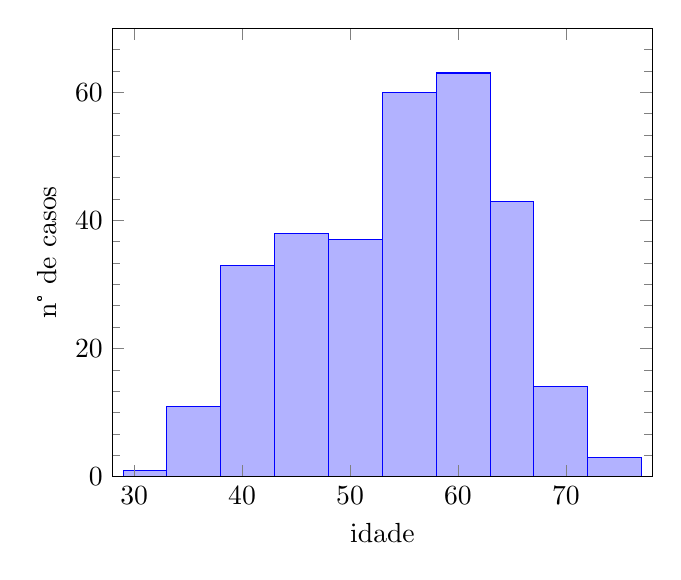
\begin{tikzpicture}
            \begin{axis}[
                xlabel={idade},
                ylabel={n° de casos},
                ymin=0, ymax=70,
                xmin=28, xmax=78,
                minor y tick num = 5,
                area style,
                ]
                \addplot+[ybar interval, mark=no] plot coordinates { (29, 1) (33, 11) (38, 33) (43, 38) (48, 37) (53, 60) (58, 63) (63, 43)  (67, 14)  (72, 3)  (77, 3)};
            \end{axis}
        \end{tikzpicture}
        \legend{Fonte: Produzido pelos próprios autores}
    \end{figure}

    Com o histograma, podemos observar uma ocorrência maior de casos em pessoas com 
    faixa etária entre 50 à 65 anos. A presença de casos para pessoas abaixo de 30 
    anos e acima dos 80 anos é quase nula.

    \begin{figure}[H]
      \centering
      \caption{Histograma do colesterol}  
      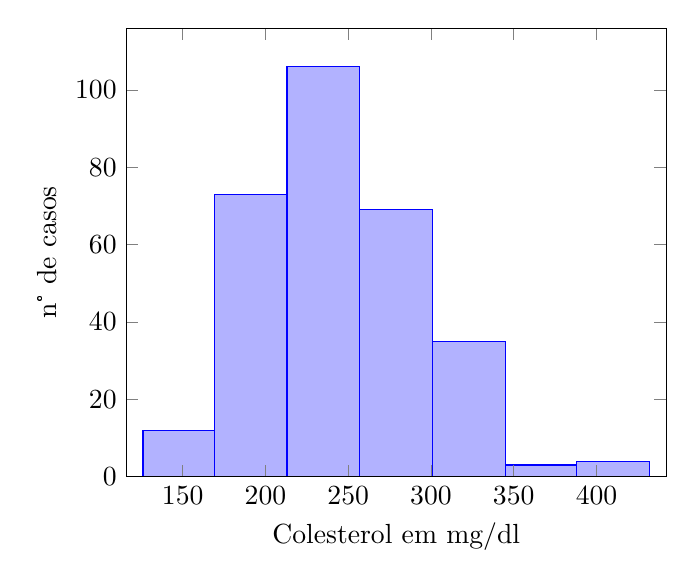
\begin{tikzpicture}
          \begin{axis}[
              xlabel={Colesterol em mg/dl},
              ylabel={n° de casos},
              ymin=0, ymax=116,
              xmin=116, xmax=442,
              area style,
              ]
              \addplot+[ybar interval, mark=no] plot coordinates { (126, 12) (169, 73) (213, 106) (257, 69) (301, 35) (345, 3) (388, 4) (432, 0)};
          \end{axis}
      \end{tikzpicture}
      \legend{Fonte: Produzido pelos próprios autores}
    \end{figure}

    \begin{figure}[H]
      \centering
      \caption{Histograma do pressão sanguínea repouso }  
      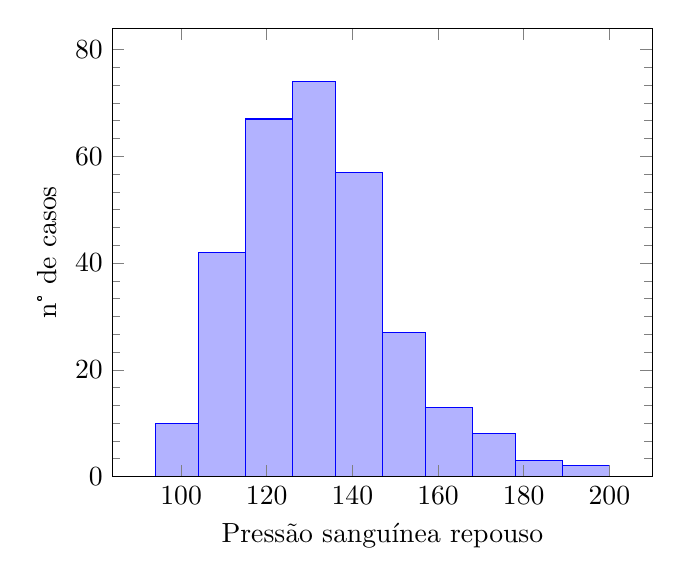
\begin{tikzpicture}
          \begin{axis}[
              xlabel={Pressão sanguínea repouso},
              ylabel={n° de casos},
              ymin=0, ymax=84,
              xmin=84, xmax=210,
              minor y tick num = 5,
              area style,
              ]
              \addplot+[ybar interval, mark=no] plot coordinates { (94, 10) (104, 42) (115, 67) (126, 74) (136, 57) (147, 27) (157, 13) (168, 8) (178, 3) (189, 2) (200, 2)};
          \end{axis}
      \end{tikzpicture}
      \legend{Fonte: Produzido pelos próprios autores}
    \end{figure}

    \begin{figure}[H]
      \centering
      \caption{Histograma do pico de batimento cardiáco }  
      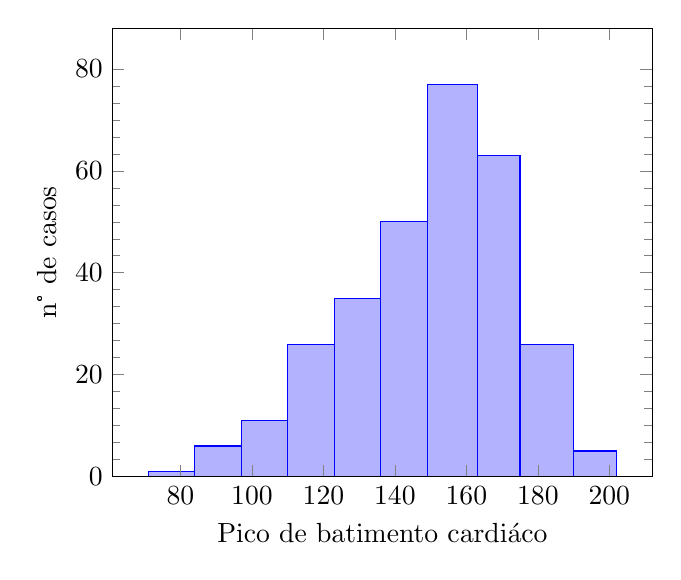
\begin{tikzpicture}
          \begin{axis}[
              xlabel={Pico de batimento cardiáco},
              ylabel={n° de casos},
              ymin=0, ymax=88,
              xmin=61, xmax=212,
              minor y tick num = 5,
              area style,
              ]
              \addplot+[ybar interval, mark=no] plot coordinates { (71, 1) (84, 6) (97, 11) (110, 26) (123, 35) (136, 50) (149, 77) (163, 63) (175, 26) (190, 5) (202, 5)};
          \end{axis}
      \end{tikzpicture}
      \legend{Fonte: Produzido pelos próprios autores}
    \end{figure}



    \nocite{sobreboxplot}
    \nocite{sobrehistograma}